Come precedentemente specificato sono state estrapolate le identit� principali intorno alle quali sviluppare la progettazione. Ci� � stato possibile grazie ad un'approfondita analisi del flusso aziendale, derivato direttamente dallo dall'analisi delle azioni e dei processi interni.\newline
Il risultato sono le cinque seguenti entit� fondamentali:

\newline\newline

\noindent\makebox[\textwidth]{\includegraphics[width=\paperwidth-1cm, trim={0 8cm 0 0}, clip]{./immagini/identit�_fondamentali.pdf}}


Gli Oggetti di propriet� del personaggio rappresentano una entit� molto importante, essi possono appartenere anche a un NPC

\begin{figure}[H]
\centering
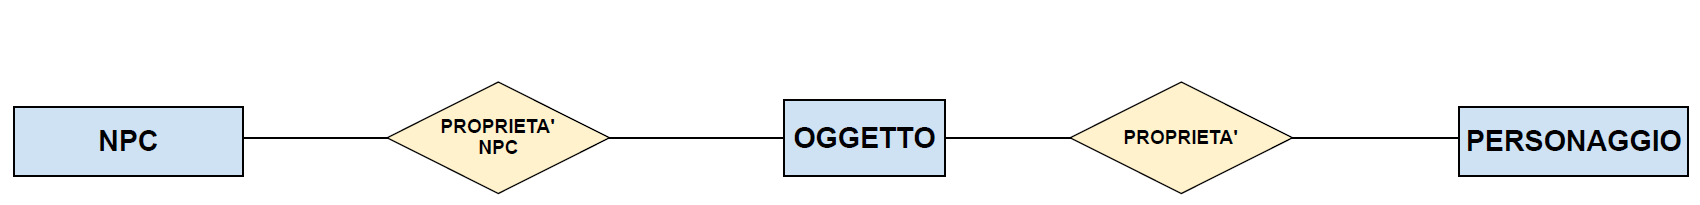
\includegraphics[width=0.7\linewidth]{./immagini/oggettotriplo.png}
\end{figure}


All'interno del gioco il personaggio interagisce con altri personaggi ed NPC come descritto nello schema dei processi interni, 
sappiamo che le interazioni di combattimento sono gestite dal Programma e non interessano la Base di Dati, tuttavia una interazione fondamentale �
la Transazione, in quanto ogni personaggio pu\`{o} vendere oggetti ad un altro o ad un NPC e risulta necessario tenere traccia di queste TRANSAZIONI

I personaggi Intraprendono e completano MISSIONI necessarie all'avanzamento nel gioco

\begin{figure}[H]
\centering
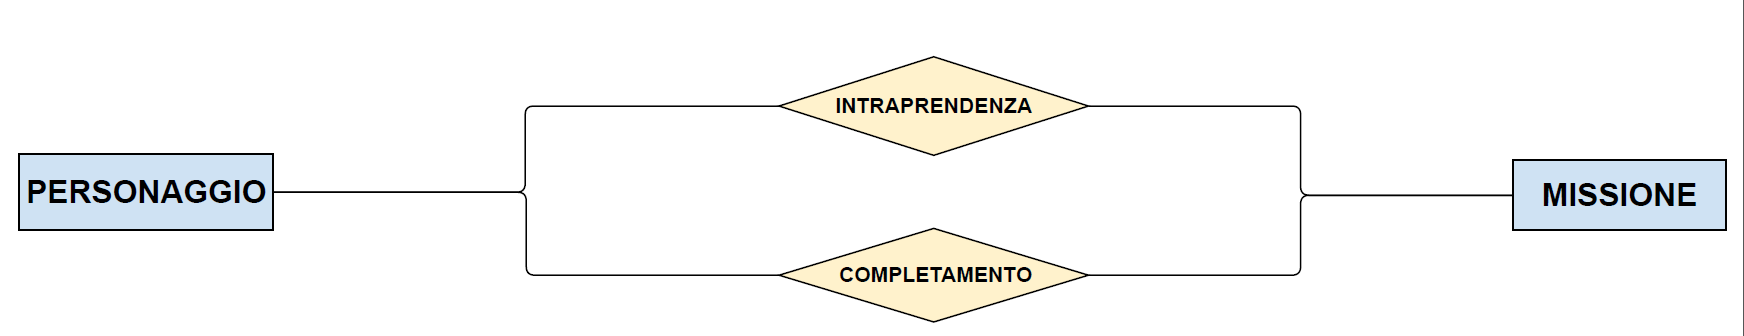
\includegraphics[width=0.7\linewidth]{./immagini/persomiss.png}
\end{figure}


Essi possono inoltre apprendere delle abilit� da degli NPC che le insegnano in cambio di denaro

\begin{figure}[H]
\centering
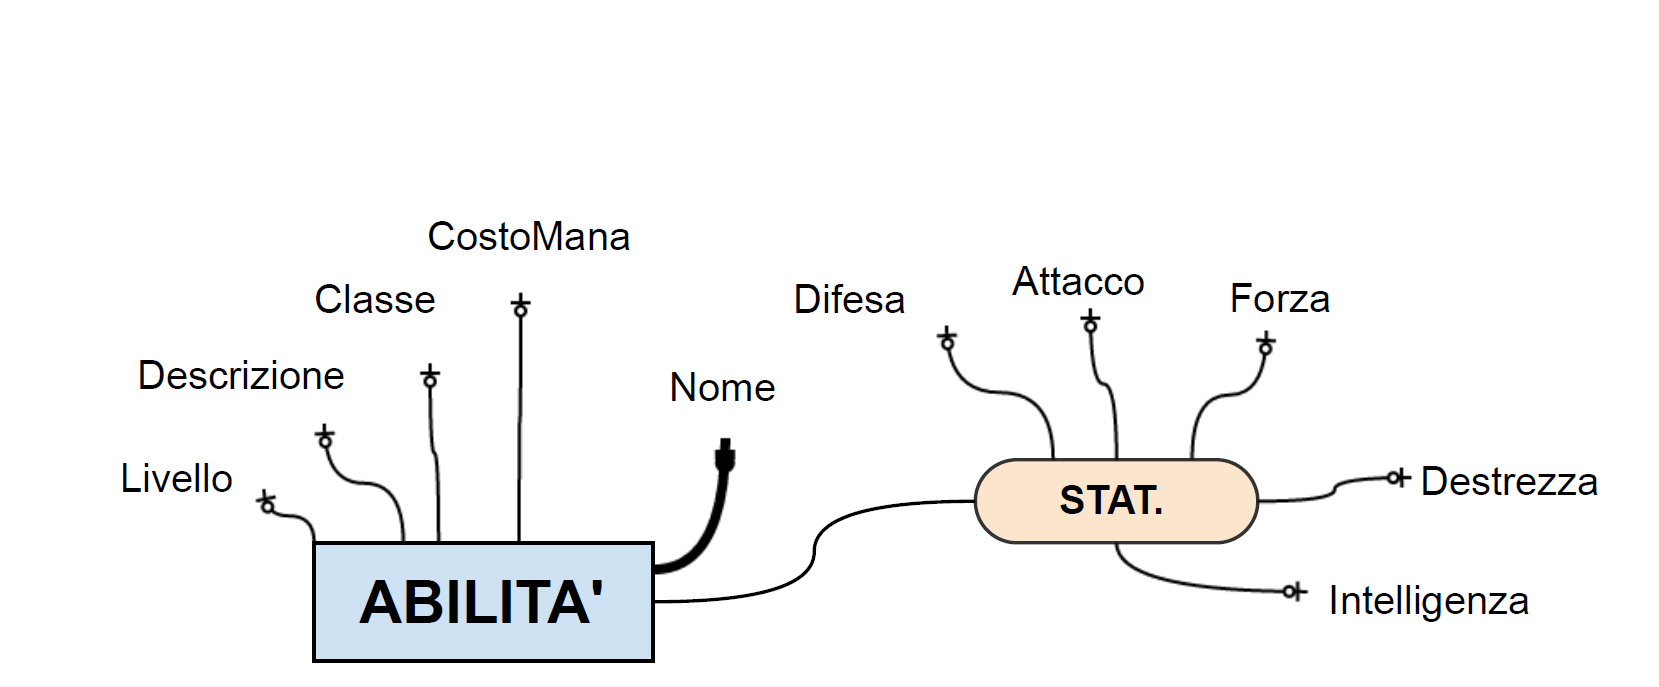
\includegraphics[width=0.7\linewidth]{./immagini/ABILITADEF.png}
\end{figure}

All'esterno del gioco vero e proprio sappiamo che ci� che accade � principalmente la creazione di personaggi dell'utente e l'acquisto di prodotti dallo store

\begin{figure}[H]
\centering
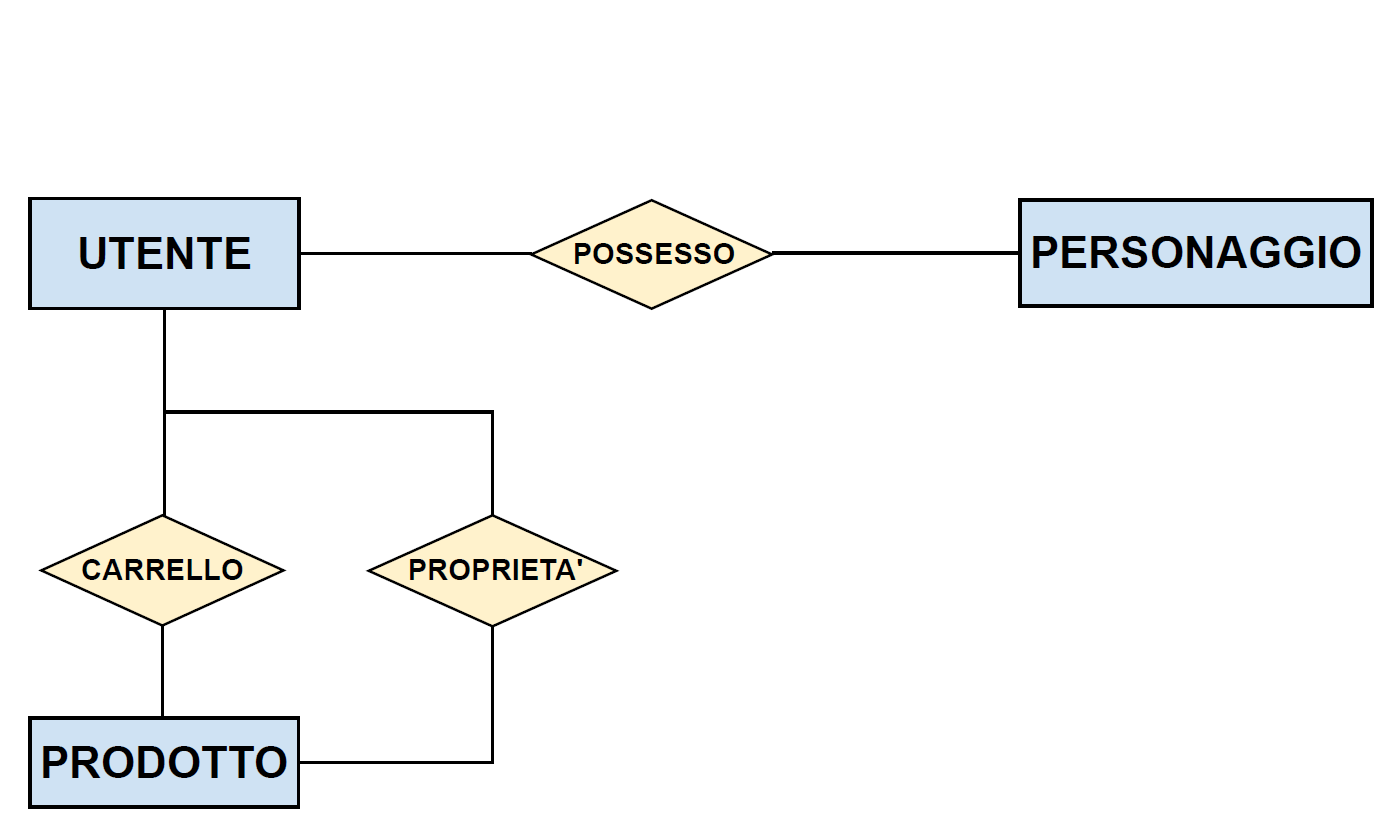
\includegraphics[width=0.7\linewidth]{./immagini/utente.png}
\end{figure}

\newpage